\documentclass[11pt]{article}
\usepackage[margin=1in]{geometry}
\usepackage{amsmath, amssymb, bm}
\usepackage{graphicx}
\usepackage{booktabs}
\usepackage{caption}
\usepackage[dvipsnames]{xcolor}
\usepackage{enumitem}
\usepackage{parskip}
\usepackage[colorlinks=true, linkcolor=RoyalBlue, urlcolor=RoyalBlue, citecolor=RoyalBlue]{hyperref}

\captionsetup{font=small, labelfont=bf}
\newcommand{\SR}{\mathrm{SR}}
\newcommand{\code}[1]{\texttt{#1}}

\title{\vspace{-2.2em}\textbf{Cointegration Statistical Arbitrage on US Equities:\\
A Null Result, a Real Edge, and the Statistics that Tell Them Apart}}
\author{Saeed Mohseni}
\date{\today}

\begin{document}
\maketitle
\vspace{-1.5em}

\begin{abstract}
\noindent
This report builds a reproducible pipeline for cointegration-based pairs trading and applies it to two
US-equity universes over 2013--2024. In the semiconductor sector, no pair is cointegrated once the screen
is corrected for multiple testing, and the best of 210 searched strategies deflates to a Sharpe of
\textbf{0.21} --- indistinguishable from luck. On a small set of economically motivated pairs chosen in
advance, the same pipeline finds a genuine edge: a Mastercard/Visa (MA/V) spread returns a Sharpe of
\textbf{1.26} ($+11.4\%$ per year, growing \$100k to \$327k) with a probabilistic Sharpe ratio of
\textbf{1.00} and a deflated Sharpe of \textbf{0.97}. The point of the exercise is not the strategy but the
discipline that separates the two outcomes: false-discovery-rate screening, walk-forward out-of-sample
backtesting, and significance tests that pay for selection bias.
\end{abstract}

\begin{center}
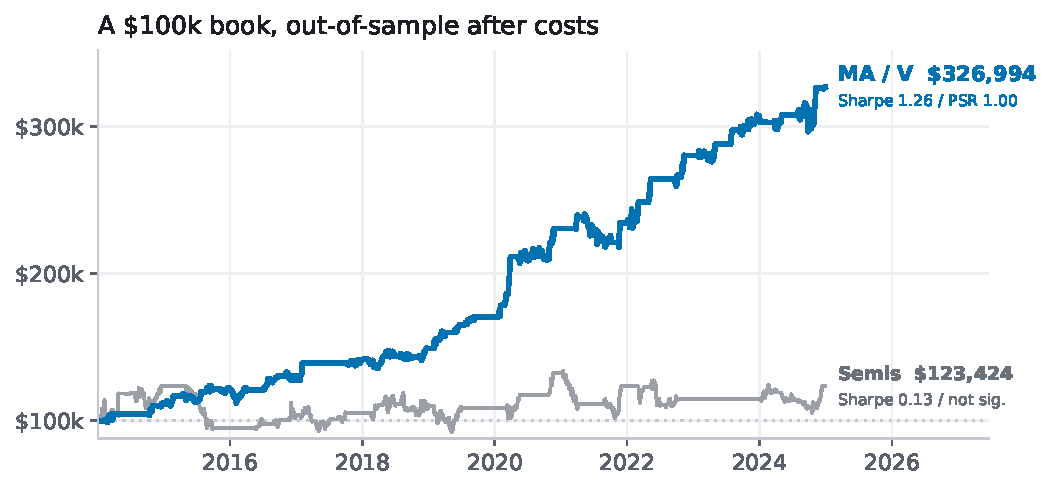
\includegraphics[width=0.82\linewidth]{figures/fig_hero.pdf}
\captionof{figure}{A \$100k book traded out-of-sample after costs. Both equity curves rise, but only MA/V
survives significance testing.}
\end{center}

% ============================================================
\section{Introduction}
Pairs trading rests on a simple idea. When two companies are economically tied, their share prices tend to
move together, and the gap between them --- the spread --- tends to return to a stable level. A trader can
sell the spread when it widens and buy it back when it closes, in principle earning a return that does not
depend on the market's overall direction.

The difficulty is that most apparent edges of this kind do not survive contact with reality. A backtest
can look profitable because it quietly used information that would not have been available at the time,
because it ignored the cost of trading, or simply because enough pairs were tried that one was bound to
look good by chance. This report asks a deliberately plain question: do cointegration pairs trades survive
realistic costs and rigorous significance testing? To answer it I built a pipeline that screens for
cointegration with a multiple-testing correction, trades the spread walk-forward with costs, and judges
every result with tests that account for both sampling noise and the number of strategies searched.

The answer depends on where one looks. In the semiconductor sector nothing survives, and the result is a
clean null. On a short list of economically motivated pairs chosen beforehand, one strategy --- long/short
Mastercard against Visa --- is genuinely profitable and statistically significant. Section~2 develops the
method, Section~3 describes the data, and Sections~4--6 present the two results and what separates them.

% ============================================================
\section{Methodology}
The pipeline is built from standard components. This section states each one briefly and gives the
reasoning behind it.

\subsection{Cointegration and the Engle--Granger test}
A price series behaves much like a random walk: it has a unit root and wanders without returning to any
particular level. A tradeable spread has to be the opposite --- stationary, pulled back toward its mean.
Engle--Granger tests for this in two steps: regress one log price on the other to obtain a hedge ratio
$\beta$, then apply the Augmented Dickey--Fuller test to the residual $s_t = y_t - (\alpha + \beta x_t)$
(the null is a unit root, so a small $p$-value means the spread is stationary and the pair is
cointegrated).

Correlation and cointegration are easy to confuse, but they are not the same. Correlation describes
returns moving together day to day; cointegration is a property of the price \emph{levels} --- that some
fixed combination of them stays stationary. A pairs trade needs the second, because only a stationary
spread has a mean to revert to. High correlation without cointegration is common, and, as Section~4 shows,
actively misleading.

\subsection{Multiple testing and the false discovery rate}
Screening many pairs creates a subtler problem. Testing $m=\binom{n}{2}$ pairs at the $5\%$ level produces
about $0.05\,m$ false positives even when nothing is truly cointegrated, so the raw count of ``significant''
pairs says very little. The Benjamini--Hochberg procedure rejects the ordered $p$-values up to the largest
$k$ with $p_{(k)} \le \tfrac{k}{m}\alpha$, which controls the expected \emph{fraction} of false discoveries
among the pairs it flags --- in effect scaling the bar by how many tests were run.

\subsection{Signal: half-life, z-score, and bands}
Given a cointegrated pair, the spread's speed of mean reversion comes from an AR(1)/Ornstein--Uhlenbeck fit
$\Delta s_t = a + b\,s_{t-1} + \varepsilon_t$, with half-life $-\ln 2 / b$; this sets the horizon the
strategy trades on. Positions are driven by the z-score $z_t = (s_t - \mu_s)/\sigma_s$: enter when the
spread is stretched beyond an entry band and exit as it returns toward the mean, with a gap between the two
bands so the position does not flip on small fluctuations.

\subsection{Backtest: no look-ahead and costs}
The backtest is built to avoid the two ways a track record lies. PnL uses the \emph{lagged} position,
$\text{gross}_t = \text{pos}_{t-1}(s_t - s_{t-1})$, so that a position chosen at today's close earns the
next day's move rather than today's --- letting today's position earn today's move would be look-ahead.
Every change in position pays a cost proportional to turnover $|\Delta \text{pos}_t|$. Evaluation is
walk-forward: $\beta$ and the spread's mean and standard deviation are estimated on a training window, the
next block is traded out-of-sample with those fixed parameters, and the window rolls forward. Because each
trade uses only earlier data, the concatenated result is a genuine out-of-sample record.

\subsection{Significance: the probabilistic and deflated Sharpe ratios}
Two effects can make a Sharpe ratio misleading. The first is ordinary sampling error: a Sharpe estimated
from a few years of noisy, non-normal returns carries a wide margin of error, which the probabilistic
Sharpe ratio makes explicit,
$$\mathrm{PSR}=\Phi\!\left(\frac{(\widehat{\SR}-\SR^{*})\sqrt{n-1}}
{\sqrt{1-\gamma_3\widehat{\SR}+\tfrac{\gamma_4-1}{4}\widehat{\SR}^2}}\right),$$
the probability that the true Sharpe exceeds a benchmark $\SR^{*}$, given sample size, skew, and kurtosis.
The second effect is selection: the best of many strategies is biased upward even with no skill. The
deflated Sharpe corrects for this by setting $\SR^{*}$ to the expected maximum of $N$ skill-less trials, so
a strategy is only credited to the extent it beats what a search of that size would produce by chance.

\subsection{Dynamic hedge: the Kalman filter}
The static hedge fits a single $\beta$. Because real relationships drift, the pipeline also offers a
time-varying hedge: treating $(\alpha_t, \beta_t)$ as a random-walk state observed through
$y_t = \alpha_t + \beta_t x_t + v_t$, a Kalman filter estimates the hedge online, and its one-step forecast
error serves as a look-ahead-free spread. The added complexity is worth it only when the relationship
actually moves; on a stable pair a dynamic hedge tends to chase noise and absorb the signal, a point
Section~6 returns to.

% ============================================================
\section{Data}
The study uses split- and dividend-adjusted daily closes from 2013 to 2024 --- roughly 3{,}000 trading
days --- aligned to a common calendar so that every cross-sectional observation is complete. Two universes
are examined. The first is the semiconductor sector: twenty large-cap names plus the SMH and SOXX ETFs, a
group chosen because its members share demand drivers and so are a natural place to look for
cointegration. The second is a set of fourteen names forming seven pre-declared economic pairs (MA/V,
KO/PEP, XOM/CVX, HD/LOW, GS/MS, WMT/TGT, GLD/IAU), each pairing two companies in the same business. These
were fixed in advance on economic grounds; they were not selected by mining the screen for whatever looked
most significant, which matters for the significance analysis in Section~5.

% ============================================================
\section{Results A --- Semiconductors: a null}
Of the 210 semiconductor pairs, none survive the false-discovery-rate correction. Ten clear the raw $5\%$
bar --- almost exactly the $\approx 10$ that chance alone predicts --- and all of them fall away once the
correction is applied. Trading the tightest pair, AMAT/LRCX, out-of-sample earns a Sharpe of only $0.13$
(probabilistic Sharpe $0.67$), and searching all 210 pairs and keeping the best gives a Sharpe of $0.54$
against a no-skill benchmark of $0.78$, for a deflated Sharpe of \textbf{0.21}.

\begin{center}
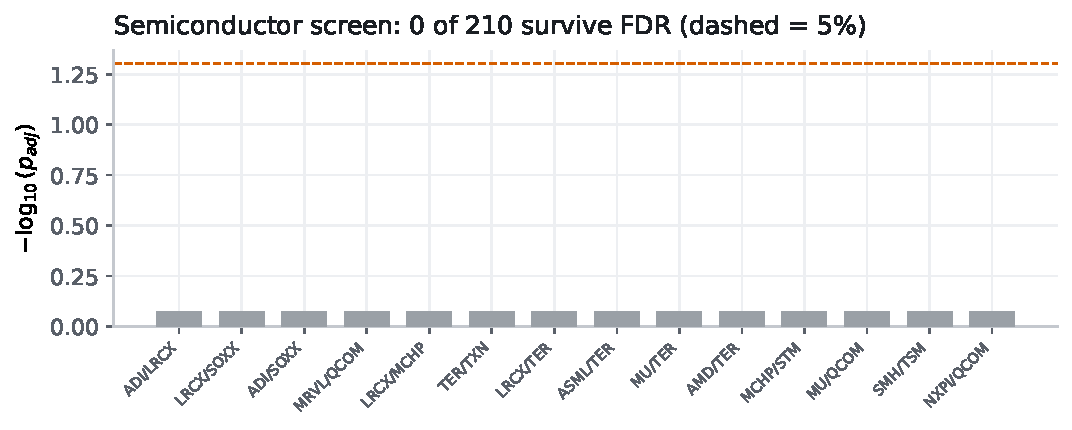
\includegraphics[width=0.70\linewidth]{figures/fig_screen_semis.pdf}\\[4pt]
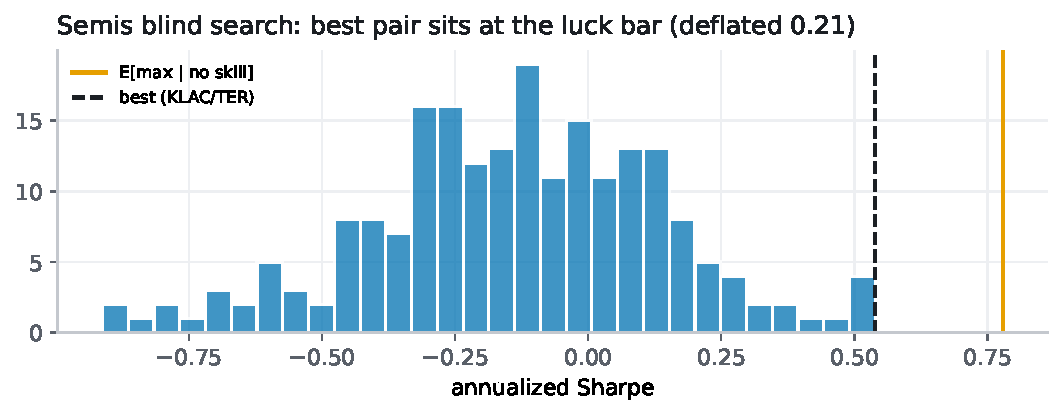
\includegraphics[width=0.72\linewidth]{figures/fig_deflated.pdf}
\captionof{figure}{Top: no semiconductor pair clears the FDR threshold. Bottom: the best of a blind
210-pair search sits at the luck bar and deflates to 0.21.}
\end{center}

A null of this kind is informative rather than disappointing. Over this period, and after the
correction, the semiconductor sector offered no pairs-trading edge --- and the pairs that looked most
promising on a raw screen were no better than the best a random search would turn up. The SMH/SOXX case
makes the mechanism concrete: two funds tracking almost the same basket are nearly perfectly correlated in
returns, yet not cointegrated, because small differences in fees and dividend timing let the ratio of
their prices drift apart over a decade. Correlation is not enough.

% ============================================================
\section{Results B --- Economic pairs: a real edge}
Screening the fourteen-name universe, only two pairs survive the correction, and both pair Walmart with a
gold ETF --- combinations with no economic reason to move together, and a reminder that a screen's smallest
$p$-values can be coincidental. The tradeable result comes instead from a pair chosen in advance. Traded
walk-forward after costs, \textbf{MA/V} (Mastercard against Visa) earns a Sharpe of \textbf{1.26}
($+11.4\%$ per year; \$100k grows to \$327k), is profitable in all eleven years, and has a $95\%$ bootstrap
confidence interval of $[0.78,\,1.79]$ with a probabilistic Sharpe near $1.00$. It stays significant across
the entire cost-and-band grid, and deflating against the seven pre-declared pairs leaves a Sharpe of
\textbf{0.97}.

\begin{center}
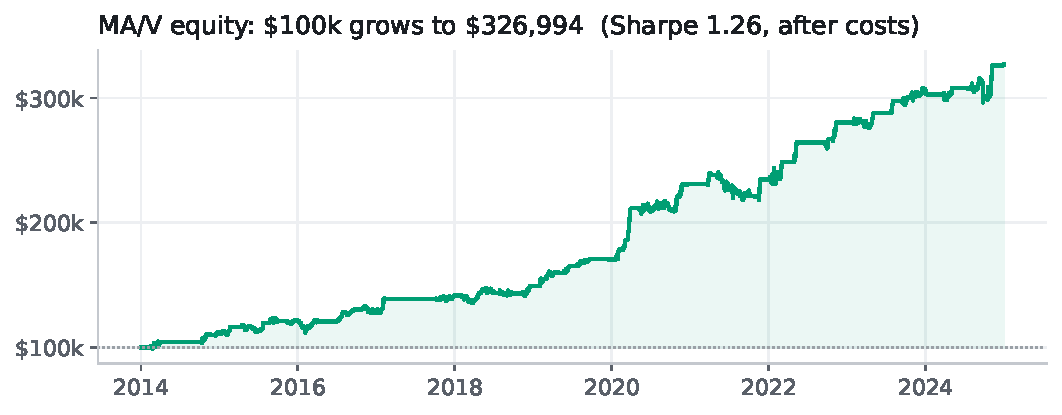
\includegraphics[width=0.72\linewidth]{figures/fig_mav_equity.pdf}\\[4pt]
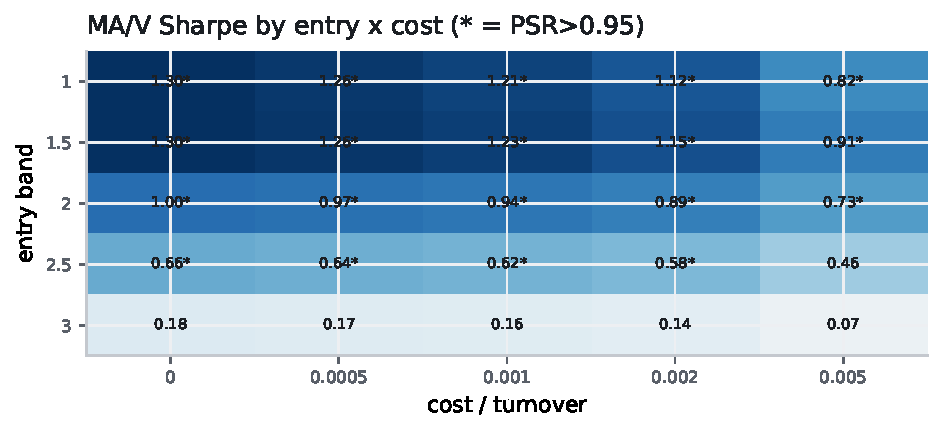
\includegraphics[width=0.60\linewidth]{figures/fig_mav_robust.pdf}
\captionof{figure}{Top: MA/V grows \$100k to \$327k out-of-sample. Bottom: the Sharpe is significant across
essentially the whole cost/entry grid.}
\end{center}

\begin{table}[h]\centering\small
\begin{tabular}{@{}lrr@{}}
\toprule
& \textbf{Semiconductors (blind search)} & \textbf{MA/V (pre-declared)} \\
\midrule
Best / pair Sharpe        & 0.54 (KLAC/TER) & 1.26 \\
Luck benchmark $\SR^{*}$  & 0.78            & --- \\
PSR (vs.\ 0)              & ---             & 1.00 \\
\textbf{Deflated Sharpe}  & \textbf{0.21}   & \textbf{0.97} \\
\bottomrule
\end{tabular}
\captionof{table}{The same significance machinery, opposite verdicts.}
\end{table}

The contrast with the semiconductor search is the central finding. There, the best of 210 pairs deflated to
0.21 precisely because it was the winner of a large search. MA/V was fixed beforehand and measured against
only a short list, so it pays almost no selection penalty and its deflated Sharpe holds at 0.97. The dollar
figure is best read as illustration: it assumes a fixed notional and frictionless compounding, and the case
for the strategy rests on the Sharpe and its significance, not on the headline total.

% ============================================================
\section{Discussion}
The two results point to the same lesson. The profitable, defensible strategy did not come from mining a
large universe for the best-looking pair; it came from a single hypothesis formed in advance and then
tested out of sample. The deflated Sharpe is what makes that distinction measurable --- it is the gap
between the semiconductor search at 0.21 and the pre-declared pair at 0.97.

The dynamic-hedge experiment makes a related point about matching a method to its problem. A Kalman filter
that lets the hedge ratio drift helped on AMAT/LRCX, whose relationship re-rated over the decade, but
underperformed a static hedge on MA/V, whose ratio was essentially constant; there the extra flexibility
only added turnover and absorbed the signal. Choosing when to use a tool mattered more than the tool
itself.

Several limitations bound these conclusions. The null rests on a single sector and the positive result on
a short list of pre-declared pairs, so a broader study would test more of each. The data are daily and the
cost model is a flat charge on turnover, so nothing here reflects intraday execution or market impact. The
evaluation covers 2013--2024 only, and while MA/V survives every test applied here, its performance in the
years since would be the real confirmation. Two natural extensions --- PCA-based residual reversion in the
style of Avellaneda and Lee, and Johansen's multivariate cointegration --- would generalize the two-asset
case to baskets.

% ============================================================
\section{Conclusion}
This project built an end-to-end, reproducible pipeline for cointegration-based pairs trading and tested
it under realistic conditions. Pairs are screened for cointegration with a correction for multiple
testing, the resulting spreads are traded out of sample with transaction costs, and each result is judged
with significance tests that account for both sampling noise and the number of strategies searched.
Applied across different equity universes, the study shows that whether a pairs trade holds up depends
far less on the trading rule than on the discipline around it: honest screening, no look-ahead, and a
correction for selection bias are what separate a genuine edge from one that only looks real. The lasting
contribution is that framework --- a method that measures a strategy's significance rather than assuming
it, and reports the outcome plainly whether or not an edge is found.

% ============================================================
\begin{thebibliography}{9}
\small
\bibitem{eg} Engle, R.F. \& Granger, C.W.J. (1987). Co-integration and error correction. \emph{Econometrica}.
\bibitem{bh} Benjamini, Y. \& Hochberg, Y. (1995). Controlling the false discovery rate. \emph{JRSS-B}.
\bibitem{psr} Bailey, D. \& L\'opez de Prado, M. (2014). The deflated Sharpe ratio. \emph{J.\ Portfolio Mgmt}.
\bibitem{chan} Chan, E. (2013). \emph{Algorithmic Trading: Winning Strategies and Their Rationale}. Wiley.
\end{thebibliography}

\end{document}
